\section{Navigation Learning Setup}
\begin{figure*}[t]
\centering
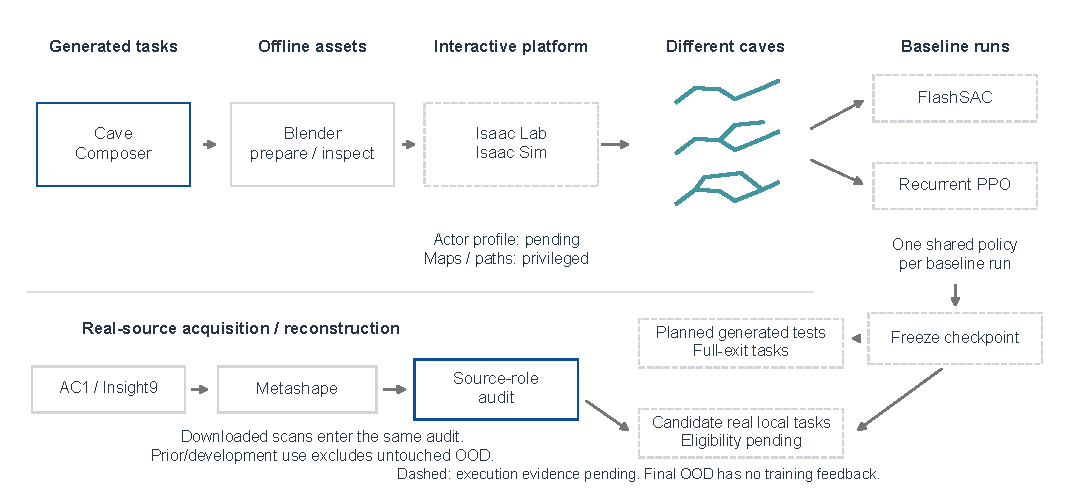
\includegraphics[width=\textwidth]{figures/generated/cavern_framework.pdf}
\caption{Planned experimental architecture. Cave Composer and offline Blender
processing feed distinct cave instances in the external Isaac Lab/Isaac Sim
platform. FlashSAC and recurrent visual PPO are alternative baseline runs;
each run is to use one policy shared across caves. The planned evaluation uses
generated full-exit tasks and candidate real-source local tasks, whose source
eligibility remains unresolved. Real sources
have an audited role before use, and the final-test branch has no feedback
to training. Dashed components require platform evidence; no rendered
miniature represents an Isaac execution screenshot.}
\label{fig:framework}
\end{figure*}
\subsection{Simulation platform and scene integration}
The collaborator reports an underwater visual-navigation platform based on
Isaac Lab. Its configuration, active training manifest and execution logs
are not yet available in this workspace. The local handoff copies verified
task packs to a new snapshot, preserves their scene splits and locks hashes.
A separate smoke test actually ran two different final cave meshes in the
existing Isaac Sim 5.0 installation, with 80\,m-separated instance origins.
Reset positions, static nonconvex triangle collision and namespace-local wall
probes pass. Synchronized 1280$\times$720 RGB pairs use the task-pack 0.12\,m
baseline and intrinsics. An initial dark-image attempt is retained; diagnostic
lamp exposure was corrected before the final check. The test uses direct USD
mesh construction, not Isaac Lab, a vehicle controller or a learned policy.
It does not validate all eight assets in the simulator. Each status distinguishes implementation,
geometry, adapter checks, simulator execution and policy evaluation.

For heterogeneous parallel training, an instance must reference its own cave
asset and task, rather than instantiate the same cave under different IDs.
A proposed sampler selects a cave uniformly and then a task within that cave.
All selected caves share a common policy for a given algorithm, configuration
and training seed. Scene identity is logging metadata, not a selector for
cave-specific policies. Per-instance transforms must move meshes, reset poses,
goals and cameras consistently.

\subsection{Observations and actions}
Historical packs specify stereo RGB sensors but leave goal conditioning and
actions unspecified. Later collaborator descriptions also mention goal or
exit instructions, IMU, pressure, previous actions and localization. The
new profile records these differences instead of modifying historical packs.
All fields of the proposed integration remain \texttt{UNCONFIRMED} until
the actual platform configuration is supplied.

Our provisional profile pairs stereo RGB with a relative goal in the body
frame, inertial and pressure measurements, and the previous action. Computing
the relative goal from simulator ground-truth pose makes this a
\emph{localization-assisted} condition, not RGB-only navigation. Global maps,
construction routes and witness paths remain privileged. The action proposal
is a normalized six-dimensional body-velocity command; actuator conversion,
limits, timing and underwater vehicle dynamics require platform confirmation.
No control or sensor-accuracy result follows from writing this interface.

\subsection{Learning baselines and task configuration}
FlashSAC and recurrent visual PPO are planned as separate baselines, each with
one cross-cave policy. Their visual encoders, memory states, optimizer settings,
normalizers and inference rules must be versioned in each imported run receipt.
The planned experiments change training
environment conditions within one baseline before comparing across baselines.
A handoff records scene and source group, assets, units, pose convention,
robot envelope, resets, goals and task budget. Evaluation receipts identify
the frozen checkpoint, data version and every scheduled episode, including
episodes not executed. Missing data never becomes a zero or an omitted failure.
The actual Isaac Lab and vehicle configuration, remaining asset-instance tests,
and matched training/evaluation receipts are still pending.
